\documentclass{article}
\usepackage[utf8]{inputenc}
\usepackage{tabularx}
\usepackage{booktabs}
\usepackage{verbatim}
\usepackage{pgf}
\usepackage{pgfplots}
\DeclareUnicodeCharacter{2212}{−}
\usepgfplotslibrary{groupplots,dateplot}
\usetikzlibrary{patterns,shapes.arrows}
\pgfplotsset{compat=newest}
\pgfplotsset{
  log ticks with fixed point,
}
\begin{document}

%
%\begin{equation}
%    \resizebox{0.9\hsize}{!}{
%    $  \bar{A} = 0.03125 \tanh{\left(0.0428571428571429 r - 0.0428571428571429 \right)} + 0.03125 \tanh{\left(0.0428571428571429 r - 0.0378571428571429 \right)} + 0.03125 \tanh{\left(0.0428571428571429 r - 0.0328571428571429 \right)} + 0.03125 \tanh{\left(0.0428571428571429 r - 0.0278571428571429 \right)} + 0.03125 \tanh{\left(0.0428571428571429 r - 0.0228571428571429 \right)} + 0.03125 \tanh{\left(0.0428571428571429 r - 0.0178571428571429 \right)} + 0.03125 \tanh{\left(0.0428571428571429 r - 0.0128571428571429 \right)} + 0.996719324059932 $}
%\end{equation}
%
\begin{figure}
    \centering
    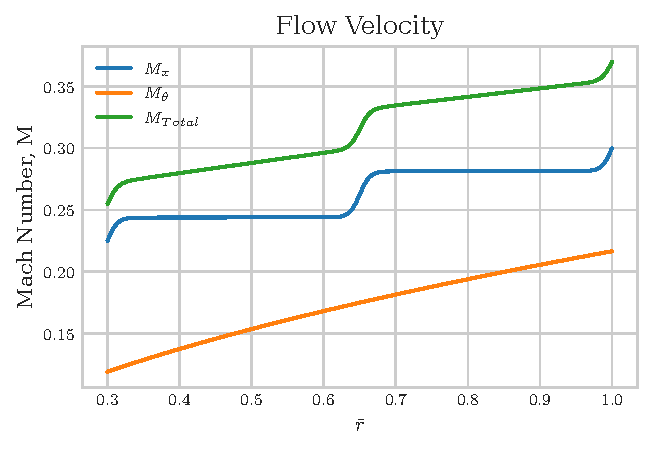
\includegraphics{tex-outputs/MachDistribution.pdf}
    \caption{Mach distribution for method of manufactured solution case}
\end{figure}

 \begin{figure}
     \centering
     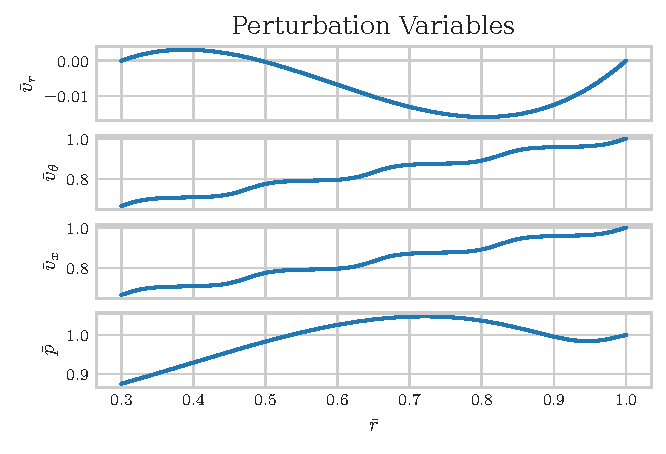
\includegraphics{tex-outputs/PerturbationVariables.pdf}
 \end{figure}

 \begin{figure}
     \centering
         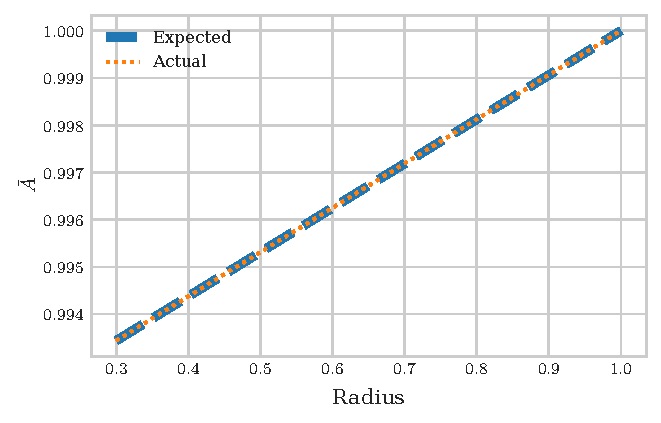
\includegraphics{tex-outputs/SoundSpeedFromIntegration.pdf}
     \caption{Speed of Sound from Integrating the Tangential Mach Number}
 \end{figure}

 \begin{figure}
     \centering
         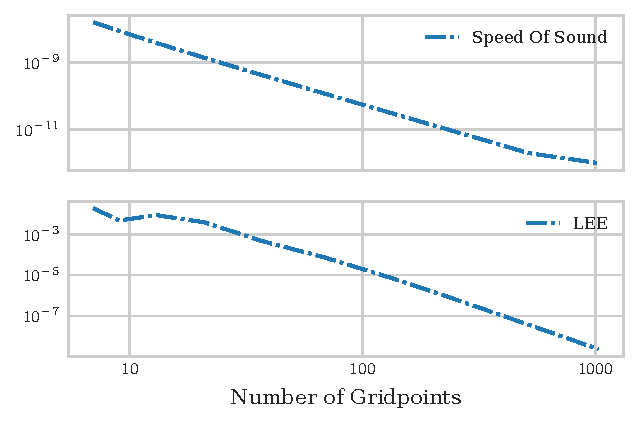
\includegraphics{tex-outputs/L2.pdf}
     \caption{L2 Norm of the Error for the MMS as a function of Grid Points}
 \end{figure}

 \begin{figure}
     \centering
         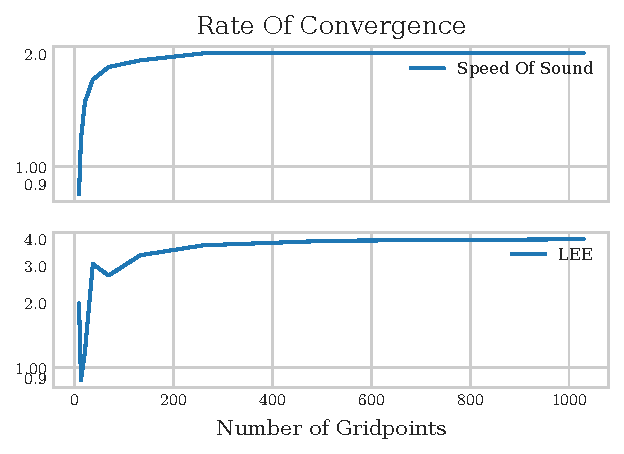
\includegraphics{tex-outputs/ROC.pdf}
     \caption{Rate of Convergence for the Speed of Sound Integration}
 \end{figure}

 \begin{figure}
         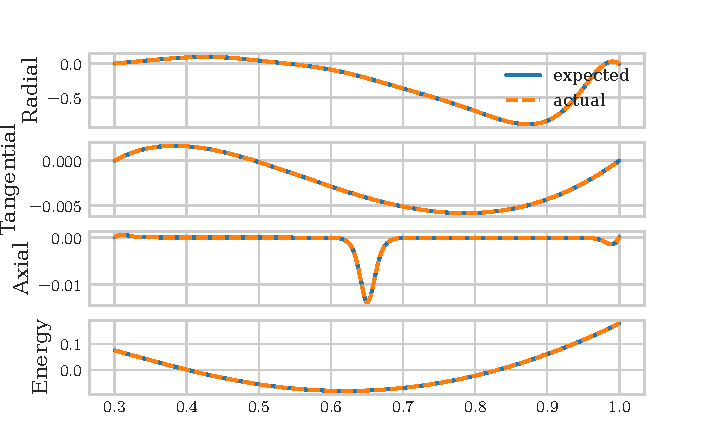
\includegraphics{tex-outputs/SourceTermData.pdf}
     \caption{Source Term Error}
 \end{figure}

%% \begin{figure}
%%     \centering
%%     % This file was created with tikzplotlib v0.9.12.
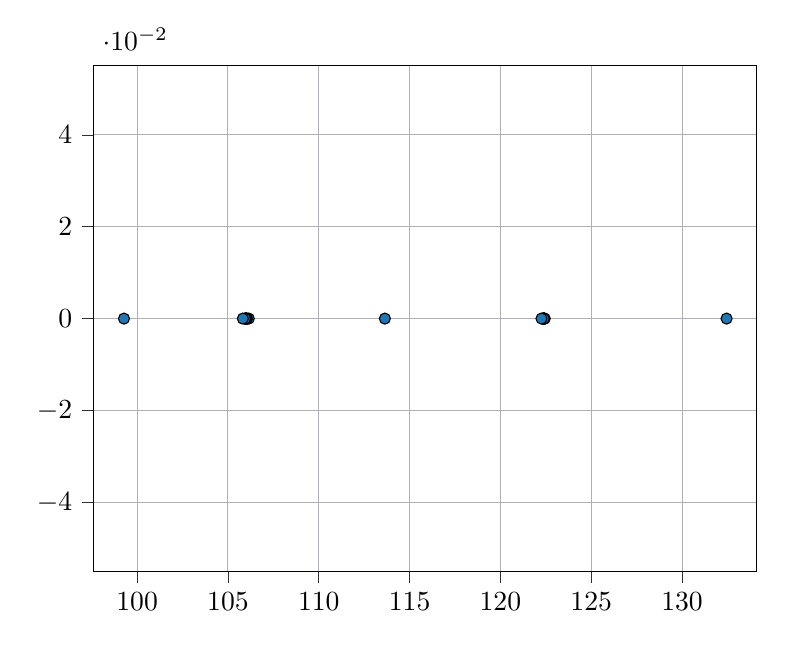
\begin{tikzpicture}

\definecolor{color0}{rgb}{0.196078431372549,0.188235294117647,0.203921568627451}
\definecolor{color1}{rgb}{0.694117647058824,0.686274509803922,0.709803921568627}
\definecolor{color2}{rgb}{0.12156862745098,0.466666666666667,0.705882352941177}

\begin{axis}[
height=8cm,
tick align=outside,
tick pos=left,
width=10cm,
x grid style={color1},
xmajorgrids,
xmin=97.6194, xmax=134.1086,
xtick style={color=color0},
y grid style={color1},
ymajorgrids,
ymin=-0.055, ymax=0.055,
ytick style={color=color0}
]
\addplot [draw=black, fill=color2, mark=*, only marks]
table{%
x  y
132.45 0
122.44 0
122.34 0
122.37 0
122.38 0
122.39 0
122.4 0
122.4 0
122.39 0
122.26 0
113.64 0
106.15 0
106.04 0
106.03 0
106.01 0
105.99 0
105.98 0
105.96 0
105.94 0
105.82 0
99.278 0
};
\end{axis}

\end{tikzpicture}

%% \end{figure}
%%
%% \begin{figure}
%%     \centering
%%     \begin{tabular}{lrr}
\toprule
{} &     REAL &  IMAG \\
\midrule
0   &  132.450 &   0.0 \\
1   &  130.390 &   0.0 \\
2   &  128.530 &   0.0 \\
3   &  126.960 &   0.0 \\
4   &  125.700 &   0.0 \\
5   &  124.730 &   0.0 \\
6   &  124.010 &   0.0 \\
7   &  123.500 &   0.0 \\
8   &  123.130 &   0.0 \\
9   &  122.870 &   0.0 \\
10  &  122.690 &   0.0 \\
11  &  122.570 &   0.0 \\
12  &  122.490 &   0.0 \\
13  &  122.440 &   0.0 \\
14  &  122.400 &   0.0 \\
15  &  122.370 &   0.0 \\
16  &  122.360 &   0.0 \\
17  &  122.350 &   0.0 \\
18  &  122.340 &   0.0 \\
19  &  122.340 &   0.0 \\
20  &  122.340 &   0.0 \\
21  &  122.340 &   0.0 \\
22  &  122.340 &   0.0 \\
23  &  122.340 &   0.0 \\
24  &  122.340 &   0.0 \\
25  &  122.340 &   0.0 \\
26  &  122.340 &   0.0 \\
27  &  122.350 &   0.0 \\
28  &  122.350 &   0.0 \\
29  &  122.350 &   0.0 \\
30  &  122.350 &   0.0 \\
31  &  122.350 &   0.0 \\
32  &  122.360 &   0.0 \\
33  &  122.360 &   0.0 \\
34  &  122.360 &   0.0 \\
35  &  122.360 &   0.0 \\
36  &  122.360 &   0.0 \\
37  &  122.360 &   0.0 \\
38  &  122.370 &   0.0 \\
39  &  122.370 &   0.0 \\
40  &  122.370 &   0.0 \\
41  &  122.370 &   0.0 \\
42  &  122.370 &   0.0 \\
43  &  122.370 &   0.0 \\
44  &  122.370 &   0.0 \\
45  &  122.380 &   0.0 \\
46  &  122.380 &   0.0 \\
47  &  122.380 &   0.0 \\
48  &  122.380 &   0.0 \\
49  &  122.380 &   0.0 \\
50  &  122.380 &   0.0 \\
51  &  122.380 &   0.0 \\
52  &  122.380 &   0.0 \\
53  &  122.380 &   0.0 \\
54  &  122.390 &   0.0 \\
55  &  122.390 &   0.0 \\
56  &  122.390 &   0.0 \\
57  &  122.390 &   0.0 \\
58  &  122.390 &   0.0 \\
59  &  122.390 &   0.0 \\
60  &  122.390 &   0.0 \\
61  &  122.390 &   0.0 \\
62  &  122.390 &   0.0 \\
63  &  122.390 &   0.0 \\
64  &  122.390 &   0.0 \\
65  &  122.390 &   0.0 \\
66  &  122.390 &   0.0 \\
67  &  122.390 &   0.0 \\
68  &  122.400 &   0.0 \\
69  &  122.400 &   0.0 \\
70  &  122.400 &   0.0 \\
71  &  122.400 &   0.0 \\
72  &  122.400 &   0.0 \\
73  &  122.400 &   0.0 \\
74  &  122.400 &   0.0 \\
75  &  122.400 &   0.0 \\
76  &  122.400 &   0.0 \\
77  &  122.400 &   0.0 \\
78  &  122.400 &   0.0 \\
79  &  122.400 &   0.0 \\
80  &  122.400 &   0.0 \\
81  &  122.400 &   0.0 \\
82  &  122.400 &   0.0 \\
83  &  122.400 &   0.0 \\
84  &  122.400 &   0.0 \\
85  &  122.400 &   0.0 \\
86  &  122.400 &   0.0 \\
87  &  122.400 &   0.0 \\
88  &  122.400 &   0.0 \\
89  &  122.400 &   0.0 \\
90  &  122.400 &   0.0 \\
91  &  122.400 &   0.0 \\
92  &  122.400 &   0.0 \\
93  &  122.400 &   0.0 \\
94  &  122.400 &   0.0 \\
95  &  122.400 &   0.0 \\
96  &  122.400 &   0.0 \\
97  &  122.400 &   0.0 \\
98  &  122.400 &   0.0 \\
99  &  122.400 &   0.0 \\
100 &  122.400 &   0.0 \\
101 &  122.400 &   0.0 \\
102 &  122.400 &   0.0 \\
103 &  122.390 &   0.0 \\
104 &  122.390 &   0.0 \\
105 &  122.390 &   0.0 \\
106 &  122.390 &   0.0 \\
107 &  122.390 &   0.0 \\
108 &  122.390 &   0.0 \\
109 &  122.390 &   0.0 \\
110 &  122.380 &   0.0 \\
111 &  122.380 &   0.0 \\
112 &  122.370 &   0.0 \\
113 &  122.360 &   0.0 \\
114 &  122.350 &   0.0 \\
115 &  122.330 &   0.0 \\
116 &  122.300 &   0.0 \\
117 &  122.260 &   0.0 \\
118 &  122.200 &   0.0 \\
119 &  122.120 &   0.0 \\
120 &  121.990 &   0.0 \\
121 &  121.820 &   0.0 \\
122 &  121.560 &   0.0 \\
123 &  121.200 &   0.0 \\
124 &  120.700 &   0.0 \\
125 &  120.030 &   0.0 \\
126 &  119.140 &   0.0 \\
127 &  118.030 &   0.0 \\
128 &  116.700 &   0.0 \\
129 &  115.200 &   0.0 \\
130 &  113.640 &   0.0 \\
131 &  112.120 &   0.0 \\
132 &  110.740 &   0.0 \\
133 &  109.560 &   0.0 \\
134 &  108.620 &   0.0 \\
135 &  107.890 &   0.0 \\
136 &  107.350 &   0.0 \\
137 &  106.960 &   0.0 \\
138 &  106.680 &   0.0 \\
139 &  106.490 &   0.0 \\
140 &  106.350 &   0.0 \\
141 &  106.260 &   0.0 \\
142 &  106.190 &   0.0 \\
143 &  106.150 &   0.0 \\
144 &  106.110 &   0.0 \\
145 &  106.090 &   0.0 \\
146 &  106.080 &   0.0 \\
147 &  106.070 &   0.0 \\
148 &  106.060 &   0.0 \\
149 &  106.060 &   0.0 \\
150 &  106.050 &   0.0 \\
151 &  106.050 &   0.0 \\
152 &  106.050 &   0.0 \\
153 &  106.040 &   0.0 \\
154 &  106.040 &   0.0 \\
155 &  106.040 &   0.0 \\
156 &  106.040 &   0.0 \\
157 &  106.040 &   0.0 \\
158 &  106.040 &   0.0 \\
159 &  106.040 &   0.0 \\
160 &  106.040 &   0.0 \\
161 &  106.030 &   0.0 \\
162 &  106.030 &   0.0 \\
163 &  106.030 &   0.0 \\
164 &  106.030 &   0.0 \\
165 &  106.030 &   0.0 \\
166 &  106.030 &   0.0 \\
167 &  106.030 &   0.0 \\
168 &  106.030 &   0.0 \\
169 &  106.030 &   0.0 \\
170 &  106.020 &   0.0 \\
171 &  106.020 &   0.0 \\
172 &  106.020 &   0.0 \\
173 &  106.020 &   0.0 \\
174 &  106.020 &   0.0 \\
175 &  106.020 &   0.0 \\
176 &  106.020 &   0.0 \\
177 &  106.020 &   0.0 \\
178 &  106.010 &   0.0 \\
179 &  106.010 &   0.0 \\
180 &  106.010 &   0.0 \\
181 &  106.010 &   0.0 \\
182 &  106.010 &   0.0 \\
183 &  106.010 &   0.0 \\
184 &  106.010 &   0.0 \\
185 &  106.010 &   0.0 \\
186 &  106.010 &   0.0 \\
187 &  106.000 &   0.0 \\
188 &  106.000 &   0.0 \\
189 &  106.000 &   0.0 \\
190 &  106.000 &   0.0 \\
191 &  106.000 &   0.0 \\
192 &  106.000 &   0.0 \\
193 &  106.000 &   0.0 \\
194 &  106.000 &   0.0 \\
195 &  105.990 &   0.0 \\
196 &  105.990 &   0.0 \\
197 &  105.990 &   0.0 \\
198 &  105.990 &   0.0 \\
199 &  105.990 &   0.0 \\
200 &  105.990 &   0.0 \\
201 &  105.990 &   0.0 \\
202 &  105.980 &   0.0 \\
203 &  105.980 &   0.0 \\
204 &  105.980 &   0.0 \\
205 &  105.980 &   0.0 \\
206 &  105.980 &   0.0 \\
207 &  105.980 &   0.0 \\
208 &  105.980 &   0.0 \\
209 &  105.970 &   0.0 \\
210 &  105.970 &   0.0 \\
211 &  105.970 &   0.0 \\
212 &  105.970 &   0.0 \\
213 &  105.970 &   0.0 \\
214 &  105.970 &   0.0 \\
215 &  105.970 &   0.0 \\
216 &  105.960 &   0.0 \\
217 &  105.960 &   0.0 \\
218 &  105.960 &   0.0 \\
219 &  105.960 &   0.0 \\
220 &  105.960 &   0.0 \\
221 &  105.960 &   0.0 \\
222 &  105.960 &   0.0 \\
223 &  105.950 &   0.0 \\
224 &  105.950 &   0.0 \\
225 &  105.950 &   0.0 \\
226 &  105.950 &   0.0 \\
227 &  105.950 &   0.0 \\
228 &  105.950 &   0.0 \\
229 &  105.950 &   0.0 \\
230 &  105.940 &   0.0 \\
231 &  105.940 &   0.0 \\
232 &  105.940 &   0.0 \\
233 &  105.940 &   0.0 \\
234 &  105.940 &   0.0 \\
235 &  105.940 &   0.0 \\
236 &  105.930 &   0.0 \\
237 &  105.930 &   0.0 \\
238 &  105.930 &   0.0 \\
239 &  105.930 &   0.0 \\
240 &  105.920 &   0.0 \\
241 &  105.920 &   0.0 \\
242 &  105.910 &   0.0 \\
243 &  105.900 &   0.0 \\
244 &  105.890 &   0.0 \\
245 &  105.880 &   0.0 \\
246 &  105.860 &   0.0 \\
247 &  105.820 &   0.0 \\
248 &  105.780 &   0.0 \\
249 &  105.710 &   0.0 \\
250 &  105.620 &   0.0 \\
251 &  105.480 &   0.0 \\
252 &  105.290 &   0.0 \\
253 &  105.020 &   0.0 \\
254 &  104.640 &   0.0 \\
255 &  104.130 &   0.0 \\
256 &  103.470 &   0.0 \\
257 &  102.620 &   0.0 \\
258 &  101.610 &   0.0 \\
259 &  100.470 &   0.0 \\
260 &   99.278 &   0.0 \\
\bottomrule
\end{tabular}

%% \end{figure}
%%
%% \begin{figure}
%%     \centering
%%     % This file was created with tikzplotlib v0.9.12.
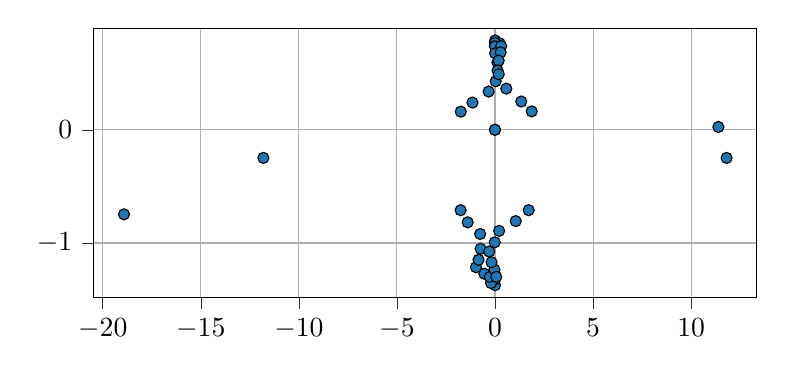
\begin{tikzpicture}

\definecolor{color0}{rgb}{0.196078431372549,0.188235294117647,0.203921568627451}
\definecolor{color1}{rgb}{0.694117647058824,0.686274509803922,0.709803921568627}
\definecolor{color2}{rgb}{0.12156862745098,0.466666666666667,0.705882352941177}

\begin{axis}[
height=5cm,
tick align=outside,
tick pos=left,
width=10cm,
x grid style={color1},
xmajorgrids,
xmin=-20.45393293861, xmax=13.34513860961,
xtick style={color=color0},
y grid style={color1},
ymajorgrids,
ymin=-1.4803407378745, ymax=0.8969239427845,
ytick style={color=color0}
]
\addplot [draw=black, fill=color2, mark=*, only marks]
table{%
x  y
0.00493032002939 0.7888664573
0.00274399605264 -1.37228325239
0 0
0.235333104789 0.76400392347
-0.00102114227909 -1.32100958537
-0.203836768749 -1.35372961458
-0.00314873885603 0.766998177369
-0.003392109022 0.736772195695
-0.546120367146 -1.27116752524
-0.266162937629 -1.2993898306
0.315615481413 0.738544875669
0.00511734307696 0.675431093693
-0.0291883807179 -1.23434923266
-0.969529687189 -1.21371700201
0.287781512337 0.683614719737
0.126251468326 0.593613930257
-0.837597044705 -1.14844270841
0.187241454813 0.610650182794
-0.176436297339 -1.16973395102
-0.732488083315 -1.05128302851
0.0629674356327 -1.29870023721
0.130109152601 0.523679011665
-0.296606952118 -1.07491888879
-0.0123825438381 -0.993935602784
0.035394238068 0.428270563326
-0.755722366351 -0.92003946127
0.19060637302 0.490045561558
-1.39157897846 -0.817213611342
0.210777487965 -0.892450595866
-18.9176115046 -0.746672628821
-1.14855622162 0.240137093615
1.34009466829 0.249607482846
1.87290508295 0.16238225419
11.3904109636 0.0247140543722
-11.8088171638 -0.248292045674
-1.75343641794 -0.71049835596
1.05815409048 -0.806591063669
-0.325225604934 0.337544455259
-1.74410627385 0.160190169508
0.57693413288 0.363509534049
11.8088171756 -0.248292044199
0 0
1.71753789017 -0.709962362132
};
\end{axis}

\end{tikzpicture}

%% \end{figure}
%%
%% \begin{figure}
%%     \centering
%%     \begin{tabular}{rrrrrrr}
\toprule
  \# &         j &     Re\{gam\} &   Im\{gam\} &  Re\{gam/ak\} &  Im\{gam/ak\} &  nz \\
\midrule
 62 &  0.015766 &    0.916376 & -0.015766 &   -0.916376 &           0 & NaN \\
 70 & -2.000000 &    0.000000 &  2.000000 &   -0.000000 &           0 & NaN \\
128 &  0.000000 &    0.000000 & -0.000000 &   -0.000000 &           0 & NaN \\
 61 &  0.600287 &   -4.901414 & -0.600287 &    4.901414 &           0 & NaN \\
 59 & -5.765258 &   -4.038264 &  5.765258 &    4.038264 &           0 & NaN \\
 64 &  0.666667 &   -2.508532 & -0.666667 &    2.508532 &           0 & NaN \\
 90 & -2.000000 &    0.000000 &  2.000000 &   -0.000000 &           0 & NaN \\
 96 & -2.000000 &    0.000000 &  2.000000 &   -0.000000 &           0 & NaN \\
 81 & -2.000000 &    0.000000 &  2.000000 &   -0.000000 &           0 & NaN \\
 77 & -2.000000 &    0.000000 &  2.000000 &   -0.000000 &           0 & NaN \\
 93 & -2.000000 &    0.000000 &  2.000000 &   -0.000000 &           1 & NaN \\
 58 &  0.091478 &  -16.043075 & -0.091478 &   16.043075 &           1 & NaN \\
 65 & -2.000000 &    0.000000 &  2.000000 &   -0.000000 &           1 & NaN \\
 60 &  1.931194 &    6.962208 & -1.931194 &   -6.962208 &           1 & NaN \\
 74 & -2.000000 &    0.000000 &  2.000000 &   -0.000000 &           1 & NaN \\
 63 &  0.666667 &    2.508532 & -0.666667 &   -2.508532 &           1 & NaN \\
 56 &  1.482415 &   16.550746 & -1.482415 &  -16.550746 &           1 & NaN \\
 54 &  0.271034 &  -27.075614 & -0.271034 &   27.075614 &           2 & NaN \\
110 & -2.000000 &    0.000000 &  2.000000 &   -0.000000 &           2 & NaN \\
 82 & -2.000000 &    0.000000 &  2.000000 &   -0.000000 &           2 & NaN \\
 68 & -2.000000 &    0.000000 &  2.000000 &   -0.000000 &           2 & NaN \\
122 & -2.000000 &    0.000000 &  2.000000 &   -0.000000 &           2 & NaN \\
 53 &  1.160191 &   27.257511 & -1.160191 &  -27.257511 &           2 & NaN \\
 57 &  0.666600 &  -19.587446 & -0.666600 &   19.587446 &           3 & NaN \\
121 & -2.000000 &    0.000000 &  2.000000 &   -0.000000 &           3 & NaN \\
 50 &  0.635024 &   38.585788 & -0.635024 &  -38.585788 &           3 & NaN \\
 49 &  1.046637 &   38.132508 & -1.046637 &  -38.132508 &           3 & NaN \\
 55 &  0.666773 &   19.587484 & -0.666773 &  -19.587484 &           3 & NaN \\
109 & -2.000000 &    0.000000 &  2.000000 &   -0.000000 &           3 & NaN \\
102 & -2.000000 &    0.000000 &  2.000000 &   -0.000000 &           3 & NaN \\
 51 &  0.346580 &  -38.041531 & -0.346580 &   38.041531 &           3 & NaN \\
 52 &  0.690092 &  -38.584396 & -0.690092 &   38.584396 &           3 & NaN \\
 48 &  0.429944 &  -48.879059 & -0.429944 &   48.879059 &           4 & NaN \\
 45 &  0.935107 &   48.934881 & -0.935107 &  -48.934881 &           4 & NaN \\
 46 &  0.466667 &  -59.657806 & -0.466667 &   59.657806 &           5 & NaN \\
 43 &  0.888435 &   59.695852 & -0.888435 &  -59.695852 &           5 & NaN \\
 47 &  0.668062 &  -57.048591 & -0.668062 &   57.048591 &           5 & NaN \\
 44 &  0.665149 &   57.048299 & -0.665149 &  -57.048299 &           5 & NaN \\
 89 & -2.000000 &    0.000000 &  2.000000 &   -0.000000 &           5 & NaN \\
 69 & -2.000000 &    0.000000 &  2.000000 &   -0.000000 &           5 & NaN \\
126 & -2.000000 &    0.000000 &  2.000000 &   -0.000000 &           5 & NaN \\
 95 & -2.000000 &    0.000000 &  2.000000 &   -0.000000 &           5 & NaN \\
115 & -2.000000 &    0.000000 &  2.000000 &   -0.000000 &           6 & NaN \\
124 & -2.000000 &    0.000000 &  2.000000 &   -0.000000 &           6 & NaN \\
 92 & -2.000000 &    0.000000 &  2.000000 &   -0.000000 &           6 & NaN \\
 42 &  0.495357 &  -70.417678 & -0.495357 &   70.417678 &           6 & NaN \\
 39 &  0.853685 &   70.445004 & -0.853685 &  -70.445004 &           6 & NaN \\
120 & -2.000000 &    0.000000 &  2.000000 &   -0.000000 &           7 & NaN \\
 80 & -2.000000 &    0.000000 &  2.000000 &   -0.000000 &           7 & NaN \\
104 & -2.000000 &    0.000000 &  2.000000 &   -0.000000 &           7 & NaN \\
101 & -2.000000 &    0.000000 &  2.000000 &   -0.000000 &           7 & NaN \\
107 & -2.000000 &    0.000000 &  2.000000 &   -0.000000 &           7 & NaN \\
 87 & -2.000000 &    0.000000 &  2.000000 &   -0.000000 &           7 & NaN \\
 40 &  0.514614 &  -80.843137 & -0.514614 &   80.843137 &           7 & NaN \\
 37 &  0.830898 &   80.864069 & -0.830898 &  -80.864069 &           7 & NaN \\
 75 & -2.000000 &    0.000000 &  2.000000 &   -0.000000 &           7 & NaN \\
 71 & -2.000000 &    0.000000 &  2.000000 &   -0.000000 &           7 & NaN \\
 98 & -2.000000 &    0.000000 &  2.000000 &   -0.000000 &           8 & NaN \\
118 & -2.000000 &    0.000000 &  2.000000 &   -0.000000 &           8 & NaN \\
 41 &  0.664166 &  -74.450882 & -0.664166 &   74.450882 &           8 & NaN \\
 38 &  0.669402 &   74.451248 & -0.669402 &  -74.451248 &           8 & NaN \\
 18 & -0.294476 &   90.829999 &  0.294476 &  -90.829999 &           8 & NaN \\
 36 &  1.633756 &  -90.822492 & -1.633756 &   90.822492 &           8 & NaN \\
 35 & -0.447360 &  -90.838753 &  0.447360 &   90.838753 &           8 & NaN \\
 17 &  1.785257 &   90.849086 & -1.785257 &  -90.849086 &           8 & NaN \\
123 & -2.000000 &    0.000000 &  2.000000 &   -0.000000 &           9 & NaN \\
119 & -2.000000 &    0.000000 &  2.000000 &   -0.000000 &           9 & NaN \\
112 & -2.000000 &    0.000000 &  2.000000 &   -0.000000 &           9 & NaN \\
 88 & -2.000000 &    0.000000 &  2.000000 &   -0.000000 &           9 & NaN \\
 84 & -2.000000 &    0.000000 &  2.000000 &   -0.000000 &           9 & NaN \\
116 & -2.000000 &    0.000000 &  2.000000 &   -0.000000 &           9 & NaN \\
 79 & -2.000000 &    0.000000 &  2.000000 &   -0.000000 &           9 & NaN \\
 78 & -2.000000 &    0.000000 &  2.000000 &   -0.000000 &           9 & NaN \\
 73 & -2.000000 &    0.000000 &  2.000000 &   -0.000000 &           9 & NaN \\
 72 & -2.000000 &    0.000000 &  2.000000 &   -0.000000 &           9 & NaN \\
 34 &  0.518513 & -101.215895 & -0.518513 &  101.215895 &           9 & NaN \\
 16 &  0.824443 &  101.231926 & -0.824443 & -101.231926 &           9 & NaN \\
117 & -2.000000 &    0.000000 &  2.000000 &   -0.000000 &          10 & NaN \\
 14 &  0.786894 &  109.545819 & -0.786894 & -109.545819 &          10 & NaN \\
 94 & -2.000000 &    0.000000 &  2.000000 &   -0.000000 &          10 & NaN \\
 32 &  0.553457 & -109.534662 & -0.553457 &  109.534662 &          10 & NaN \\
 15 &  0.662390 &  105.080999 & -0.662390 & -105.080999 &          11 & NaN \\
 31 & -1.797758 & -117.617356 &  1.797758 &  117.617356 &          11 & NaN \\
108 & -2.000000 &    0.000000 &  2.000000 &   -0.000000 &          11 & NaN \\
 13 &  3.137526 &  117.618829 & -3.137526 & -117.618829 &          11 & NaN \\
 99 & -2.000000 &    0.000000 &  2.000000 &   -0.000000 &          11 & NaN \\
 91 & -2.000000 &    0.000000 &  2.000000 &   -0.000000 &          11 & NaN \\
 33 &  0.670678 & -105.081408 & -0.670678 &  105.081408 &          11 & NaN \\
 30 &  3.049586 & -117.702709 & -3.049586 &  117.702709 &          12 & NaN \\
 29 & -1.901858 & -126.357840 &  1.901858 &  126.357840 &          12 & NaN \\
111 & -2.000000 &    0.000000 &  2.000000 &   -0.000000 &          12 & NaN \\
105 & -2.000000 &    0.000000 &  2.000000 &   -0.000000 &          12 & NaN \\
 12 & -1.717631 &  117.708704 &  1.717631 & -117.708704 &          12 & NaN \\
 11 &  3.241025 &  126.355117 & -3.241025 & -126.355117 &          12 & NaN \\
 28 &  3.223902 & -126.484343 & -3.223902 &  126.484343 &          13 & NaN \\
 27 & -1.085589 & -133.829656 &  1.085589 &  133.829656 &          13 & NaN \\
103 & -2.000000 &    0.000000 &  2.000000 &   -0.000000 &          13 & NaN \\
 97 & -2.000000 &    0.000000 &  2.000000 &   -0.000000 &          13 & NaN \\
 10 & -1.895551 &  126.488185 &  1.895551 & -126.488185 &          13 & NaN \\
 83 & -2.000000 &    0.000000 &  2.000000 &   -0.000000 &          13 & NaN \\
  9 &  2.422422 &  133.826508 & -2.422422 & -133.826508 &          13 & NaN \\
 67 &  0.000000 &    0.000000 & -0.000000 &   -0.000000 &          13 & NaN \\
 86 & -2.000000 &    0.000000 &  2.000000 &   -0.000000 &          14 & NaN \\
113 & -2.000000 &    0.000000 &  2.000000 &   -0.000000 &          15 & NaN \\
106 & -2.000000 &    0.000000 &  2.000000 &   -0.000000 &          15 & NaN \\
 25 & -0.169034 & -140.039169 &  0.169034 &  140.039169 &          15 & NaN \\
 24 &  1.516659 & -140.112196 & -1.516659 &  140.112196 &          15 & NaN \\
  6 & -0.186560 &  140.113184 &  0.186560 & -140.113184 &          15 & NaN \\
 76 & -2.000000 &    0.000000 &  2.000000 &   -0.000000 &          15 & NaN \\
127 & -2.000000 &    0.000000 &  2.000000 &   -0.000000 &          16 & NaN \\
  7 &  1.504961 &  140.037108 & -1.504961 & -140.037108 &          16 & NaN \\
114 & -2.000000 &    0.000000 &  2.000000 &   -0.000000 &          16 & NaN \\
 26 &  2.441354 & -133.927501 & -2.441354 &  133.927501 &          16 & NaN \\
 23 &  0.644401 & -144.457380 & -0.644401 &  144.457380 &          16 & NaN \\
 22 &  0.692184 & -145.000688 & -0.692184 &  145.000688 &          16 & NaN \\
  5 &  0.690054 &  144.458967 & -0.690054 & -144.458967 &          16 & NaN \\
 20 & -2.963807 & -149.851153 &  2.963807 &  149.851153 &          16 & NaN \\
  2 &  4.297141 &  149.851153 & -4.297141 & -149.851153 &          16 & NaN \\
 19 &  4.297129 & -149.851151 & -4.297129 &  149.851151 &          16 & NaN \\
  8 & -1.112563 &  133.928948 &  1.112563 & -133.928948 &          16 & NaN \\
  4 &  0.639888 &  144.998863 & -0.639888 & -144.998863 &          16 & NaN \\
  1 & -2.963795 &  149.851152 &  2.963795 & -149.851152 &          16 & NaN \\
125 & -2.000000 &    0.000000 &  2.000000 &   -0.000000 &          17 & NaN \\
  3 &  0.666660 &  146.829096 & -0.666660 & -146.829096 &          17 & NaN \\
 21 &  0.666673 & -146.829096 & -0.666673 &  146.829096 &          17 & NaN \\
 66 & -2.000000 &    0.000000 &  2.000000 &   -0.000000 &          17 & NaN \\
100 & -2.000000 &    0.000000 &  2.000000 &   -0.000000 &          21 & NaN \\
 85 & -2.000000 &    0.000000 &  2.000000 &   -0.000000 &          24 & NaN \\
\bottomrule
\end{tabular}

%% \end{figure}
%
% %\begin{tiny}
% %    \verbatiminput{../04-EVanalysis/cv.waves.dat}
% %\end{tiny}
%
% %\begin{tiny}
% %    \verbatiminput{../04-EVanalysis/gammas0007.dat}
% %\end{tiny}
%% \begin{figure}
%%     \begin{center}
%%         \begin{tikzpicture}[gnuplot]
%% generated with GNUPLOT 5.2p8 (Lua 5.3; terminal rev. Nov 2018, script rev. 108)
%% Tue 21 Sep 2021 04:42:31 PM EDT
\path (0.000,0.000) rectangle (12.500,8.750);
\gpcolor{color=gp lt color axes}
\gpsetlinetype{gp lt axes}
\gpsetdashtype{gp dt axes}
\gpsetlinewidth{0.50}
\draw[gp path] (1.320,0.985)--(11.947,0.985);
\gpcolor{color=gp lt color border}
\gpsetlinetype{gp lt border}
\gpsetdashtype{gp dt solid}
\gpsetlinewidth{1.00}
\draw[gp path] (1.320,0.985)--(1.500,0.985);
\draw[gp path] (11.947,0.985)--(11.767,0.985);
\node[gp node right] at (1.136,0.985) {$0.1$};
\draw[gp path] (1.320,2.107)--(1.410,2.107);
\draw[gp path] (11.947,2.107)--(11.857,2.107);
\draw[gp path] (1.320,2.764)--(1.410,2.764);
\draw[gp path] (11.947,2.764)--(11.857,2.764);
\draw[gp path] (1.320,3.229)--(1.410,3.229);
\draw[gp path] (11.947,3.229)--(11.857,3.229);
\draw[gp path] (1.320,3.591)--(1.410,3.591);
\draw[gp path] (11.947,3.591)--(11.857,3.591);
\draw[gp path] (1.320,3.886)--(1.410,3.886);
\draw[gp path] (11.947,3.886)--(11.857,3.886);
\draw[gp path] (1.320,4.136)--(1.410,4.136);
\draw[gp path] (11.947,4.136)--(11.857,4.136);
\draw[gp path] (1.320,4.352)--(1.410,4.352);
\draw[gp path] (11.947,4.352)--(11.857,4.352);
\draw[gp path] (1.320,4.542)--(1.410,4.542);
\draw[gp path] (11.947,4.542)--(11.857,4.542);
\gpcolor{color=gp lt color axes}
\gpsetlinetype{gp lt axes}
\gpsetdashtype{gp dt axes}
\gpsetlinewidth{0.50}
\draw[gp path] (1.320,4.713)--(11.947,4.713);
\gpcolor{color=gp lt color border}
\gpsetlinetype{gp lt border}
\gpsetdashtype{gp dt solid}
\gpsetlinewidth{1.00}
\draw[gp path] (1.320,4.713)--(1.500,4.713);
\draw[gp path] (11.947,4.713)--(11.767,4.713);
\node[gp node right] at (1.136,4.713) {$1$};
\draw[gp path] (1.320,5.835)--(1.410,5.835);
\draw[gp path] (11.947,5.835)--(11.857,5.835);
\draw[gp path] (1.320,6.492)--(1.410,6.492);
\draw[gp path] (11.947,6.492)--(11.857,6.492);
\draw[gp path] (1.320,6.957)--(1.410,6.957);
\draw[gp path] (11.947,6.957)--(11.857,6.957);
\draw[gp path] (1.320,7.319)--(1.410,7.319);
\draw[gp path] (11.947,7.319)--(11.857,7.319);
\draw[gp path] (1.320,7.614)--(1.410,7.614);
\draw[gp path] (11.947,7.614)--(11.857,7.614);
\draw[gp path] (1.320,7.864)--(1.410,7.864);
\draw[gp path] (11.947,7.864)--(11.857,7.864);
\draw[gp path] (1.320,8.080)--(1.410,8.080);
\draw[gp path] (11.947,8.080)--(11.857,8.080);
\draw[gp path] (1.320,8.270)--(1.410,8.270);
\draw[gp path] (11.947,8.270)--(11.857,8.270);
\gpcolor{color=gp lt color axes}
\gpsetlinetype{gp lt axes}
\gpsetdashtype{gp dt axes}
\gpsetlinewidth{0.50}
\draw[gp path] (1.320,8.441)--(11.947,8.441);
\gpcolor{color=gp lt color border}
\gpsetlinetype{gp lt border}
\gpsetdashtype{gp dt solid}
\gpsetlinewidth{1.00}
\draw[gp path] (1.320,8.441)--(1.500,8.441);
\draw[gp path] (11.947,8.441)--(11.767,8.441);
\node[gp node right] at (1.136,8.441) {$10$};
\gpcolor{color=gp lt color axes}
\gpsetlinetype{gp lt axes}
\gpsetdashtype{gp dt axes}
\gpsetlinewidth{0.50}
\draw[gp path] (1.320,0.985)--(1.320,8.441);
\gpcolor{color=gp lt color border}
\gpsetlinetype{gp lt border}
\gpsetdashtype{gp dt solid}
\gpsetlinewidth{1.00}
\draw[gp path] (1.320,0.985)--(1.320,1.165);
\draw[gp path] (1.320,8.441)--(1.320,8.261);
\node[gp node center] at (1.320,0.677) {$0.5$};
\gpcolor{color=gp lt color axes}
\gpsetlinetype{gp lt axes}
\gpsetdashtype{gp dt axes}
\gpsetlinewidth{0.50}
\draw[gp path] (2.383,0.985)--(2.383,8.441);
\gpcolor{color=gp lt color border}
\gpsetlinetype{gp lt border}
\gpsetdashtype{gp dt solid}
\gpsetlinewidth{1.00}
\draw[gp path] (2.383,0.985)--(2.383,1.165);
\draw[gp path] (2.383,8.441)--(2.383,8.261);
\node[gp node center] at (2.383,0.677) {$0.51$};
\gpcolor{color=gp lt color axes}
\gpsetlinetype{gp lt axes}
\gpsetdashtype{gp dt axes}
\gpsetlinewidth{0.50}
\draw[gp path] (3.445,0.985)--(3.445,8.441);
\gpcolor{color=gp lt color border}
\gpsetlinetype{gp lt border}
\gpsetdashtype{gp dt solid}
\gpsetlinewidth{1.00}
\draw[gp path] (3.445,0.985)--(3.445,1.165);
\draw[gp path] (3.445,8.441)--(3.445,8.261);
\node[gp node center] at (3.445,0.677) {$0.52$};
\gpcolor{color=gp lt color axes}
\gpsetlinetype{gp lt axes}
\gpsetdashtype{gp dt axes}
\gpsetlinewidth{0.50}
\draw[gp path] (4.508,0.985)--(4.508,8.441);
\gpcolor{color=gp lt color border}
\gpsetlinetype{gp lt border}
\gpsetdashtype{gp dt solid}
\gpsetlinewidth{1.00}
\draw[gp path] (4.508,0.985)--(4.508,1.165);
\draw[gp path] (4.508,8.441)--(4.508,8.261);
\node[gp node center] at (4.508,0.677) {$0.53$};
\gpcolor{color=gp lt color axes}
\gpsetlinetype{gp lt axes}
\gpsetdashtype{gp dt axes}
\gpsetlinewidth{0.50}
\draw[gp path] (5.571,0.985)--(5.571,8.441);
\gpcolor{color=gp lt color border}
\gpsetlinetype{gp lt border}
\gpsetdashtype{gp dt solid}
\gpsetlinewidth{1.00}
\draw[gp path] (5.571,0.985)--(5.571,1.165);
\draw[gp path] (5.571,8.441)--(5.571,8.261);
\node[gp node center] at (5.571,0.677) {$0.54$};
\gpcolor{color=gp lt color axes}
\gpsetlinetype{gp lt axes}
\gpsetdashtype{gp dt axes}
\gpsetlinewidth{0.50}
\draw[gp path] (6.634,0.985)--(6.634,8.441);
\gpcolor{color=gp lt color border}
\gpsetlinetype{gp lt border}
\gpsetdashtype{gp dt solid}
\gpsetlinewidth{1.00}
\draw[gp path] (6.634,0.985)--(6.634,1.165);
\draw[gp path] (6.634,8.441)--(6.634,8.261);
\node[gp node center] at (6.634,0.677) {$0.55$};
\gpcolor{color=gp lt color axes}
\gpsetlinetype{gp lt axes}
\gpsetdashtype{gp dt axes}
\gpsetlinewidth{0.50}
\draw[gp path] (7.696,0.985)--(7.696,8.441);
\gpcolor{color=gp lt color border}
\gpsetlinetype{gp lt border}
\gpsetdashtype{gp dt solid}
\gpsetlinewidth{1.00}
\draw[gp path] (7.696,0.985)--(7.696,1.165);
\draw[gp path] (7.696,8.441)--(7.696,8.261);
\node[gp node center] at (7.696,0.677) {$0.56$};
\gpcolor{color=gp lt color axes}
\gpsetlinetype{gp lt axes}
\gpsetdashtype{gp dt axes}
\gpsetlinewidth{0.50}
\draw[gp path] (8.759,0.985)--(8.759,8.441);
\gpcolor{color=gp lt color border}
\gpsetlinetype{gp lt border}
\gpsetdashtype{gp dt solid}
\gpsetlinewidth{1.00}
\draw[gp path] (8.759,0.985)--(8.759,1.165);
\draw[gp path] (8.759,8.441)--(8.759,8.261);
\node[gp node center] at (8.759,0.677) {$0.57$};
\gpcolor{color=gp lt color axes}
\gpsetlinetype{gp lt axes}
\gpsetdashtype{gp dt axes}
\gpsetlinewidth{0.50}
\draw[gp path] (9.822,0.985)--(9.822,8.441);
\gpcolor{color=gp lt color border}
\gpsetlinetype{gp lt border}
\gpsetdashtype{gp dt solid}
\gpsetlinewidth{1.00}
\draw[gp path] (9.822,0.985)--(9.822,1.165);
\draw[gp path] (9.822,8.441)--(9.822,8.261);
\node[gp node center] at (9.822,0.677) {$0.58$};
\gpcolor{color=gp lt color axes}
\gpsetlinetype{gp lt axes}
\gpsetdashtype{gp dt axes}
\gpsetlinewidth{0.50}
\draw[gp path] (10.884,0.985)--(10.884,7.953);
\draw[gp path] (10.884,8.261)--(10.884,8.441);
\gpcolor{color=gp lt color border}
\gpsetlinetype{gp lt border}
\gpsetdashtype{gp dt solid}
\gpsetlinewidth{1.00}
\draw[gp path] (10.884,0.985)--(10.884,1.165);
\draw[gp path] (10.884,8.441)--(10.884,8.261);
\node[gp node center] at (10.884,0.677) {$0.59$};
\gpcolor{color=gp lt color axes}
\gpsetlinetype{gp lt axes}
\gpsetdashtype{gp dt axes}
\gpsetlinewidth{0.50}
\draw[gp path] (11.947,0.985)--(11.947,8.441);
\gpcolor{color=gp lt color border}
\gpsetlinetype{gp lt border}
\gpsetdashtype{gp dt solid}
\gpsetlinewidth{1.00}
\draw[gp path] (11.947,0.985)--(11.947,1.165);
\draw[gp path] (11.947,8.441)--(11.947,8.261);
\node[gp node center] at (11.947,0.677) {$0.6$};
\draw[gp path] (1.320,8.441)--(1.320,0.985)--(11.947,0.985)--(11.947,8.441)--cycle;
\node[gp node center,rotate=-270] at (0.292,4.713) {Observed Order-of-Accuracy};
\node[gp node center] at (6.633,0.215) {$\Delta $};
\node[gp node right] at (10.479,8.107) {?};
\gpcolor{rgb color={0.000,0.502,0.502}}
\draw[gp path] (10.663,8.107)--(11.579,8.107);
\draw[gp path] (11.947,2.953)--(7.224,3.734)--(4.445,5.212)--(2.930,6.020)--(2.137,6.034)%
  --(1.732,5.886)--(1.527,5.842)--(1.423,5.836)--(1.372,5.835);
\gpsetpointsize{4.00}
\gppoint{gp mark 1}{(11.947,2.953)}
\gppoint{gp mark 1}{(7.224,3.734)}
\gppoint{gp mark 1}{(4.445,5.212)}
\gppoint{gp mark 1}{(2.930,6.020)}
\gppoint{gp mark 1}{(2.137,6.034)}
\gppoint{gp mark 1}{(1.732,5.886)}
\gppoint{gp mark 1}{(1.527,5.842)}
\gppoint{gp mark 1}{(1.423,5.836)}
\gppoint{gp mark 1}{(1.372,5.835)}
\gppoint{gp mark 1}{(11.121,8.107)}
\gpcolor{color=gp lt color border}
\draw[gp path] (1.320,8.441)--(1.320,0.985)--(11.947,0.985)--(11.947,8.441)--cycle;
%% coordinates of the plot area
\gpdefrectangularnode{gp plot 1}{\pgfpoint{1.320cm}{0.985cm}}{\pgfpoint{11.947cm}{8.441cm}}
\end{tikzpicture}
%% gnuplot variables

%%     \end{center}
%%     \caption{Absolute Value Rate of Convergence for the Source Term}
%% \end{figure}
%
\end{document}

